%%%%%%%%%%%%%%%%%%%%%%%%%%%%%%%%%%%%%%%%%
%
% (c) 2022 by Jennifer Laaser
%
% This work is licensed under the Creative Commons Attribution-NonCommercial-ShareAlike 4.0 International License. To view a copy of this license, visit http://creativecommons.org/licenses/by-nc-sa/4.0/ or send a letter to Creative Commons, PO Box 1866, Mountain View, CA 94042, USA.
%
% The current source for these materials is accessible on Github: https://github.com/jlaaser/pogil-polymers
%
%%%%%%%%%%%%%%%%%%%%%%%%%%%%%%%%%%%%%%%%%

\renewcommand{\figpath}{content/polymchem/stepgrowth/kinetics/figs}
\renewcommand{\labelbase}{step-kinetics}

\begin{activity}{Kinetics of Step-Growth Polymerizations}

\begin{instructornotes}

	This activity introduces students to key concepts related to the kinetics of step-growth polymerizations.
	
	After completing this activity, students will be able to:
			\begin{enumerate}
				\item Explain the mechanistic features of step-growth polymerizations that lead to catalyzed or un-catalyzed kinetics
				\item Describe how the molecular weight of polymers produced in step-growth polymerizations changes with time for both catalyzed and uncatalyzed polymerizations
				%\item Use information about how extent of reaction and/or molecular weight changes with time to determine whether a polymerization is catalyzed or un-catalyzed
				\item Calculate the expected molecular weight of a step-growth polymer at a given reaction time
			\end{enumerate}
	
			
	\subsection*{Activity summary:}
	\begin{itemize}
		\item \textbf{Activity type:} Learning Cycle
		\item \textbf{Content goals:} See above
		\item \textbf{Process goals:} %https://pogil.org/uploads/attachments/cj54b5yts006cklx4hh758htf-process-skills-official-pogil-list-2015-original.pdf
			\begin{itemize}
				\item Interpreting chemical structures and reaction schemes
				\item Representing quantitative relationships in both equations and graphs
				\item Linking concepts to derive a key result
				\item Written and oral communication of reasoning
			\end{itemize}
		\item \textbf{Duration:} approx. 50 minutes
		\item \textbf{Instructor preparation required:} none beyond knowledge of relevant content
		\item \textbf{Related textbook chapters:}
			\begin{itemize}
				\item \emph{Polymer Chemistry} (Hiemenz \& Lodge), 2nd ed.: sections 2.2.3 and 2.3
				\item \emph{Introduction to Polymers} (Young \& Lovell), 3rd ed.: section 3.2.2.3
			\end{itemize}
	\end{itemize}

\end{instructornotes}

	%\textbf{Focus question:} Put a central question for the students to consider through this exercise here.

\begin{model}[A Simple Step-Growth Reaction]
\label{\labelbase:mdl:simple}

	The key reaction in a step-growth polymerization is the reaction of an ``A'' functional group with a ``B'' functional group to form an ``ab'' bond:
	
	\centerline{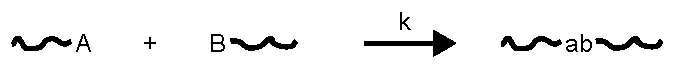
\includegraphics[width=0.7\textwidth]{\figpath/Model1_rxn}}
	
	The rate of this reaction is determined by the rate constant $k$.

\end{model}


\begin{ctqs}

	\question How many molecules must come together for this reaction to take place?
	
		\begin{solution}[0.5in]{}
			2
		\end{solution}
	
	\question Based on your answer to the previous question, explain, in 1-2 complete sentences, why it is appropriate to describe this reaction as a \emph{bimolecular} reaction.
	
		\begin{solution}[1in]{}
			Bimolecular reactions are reactions in which two molecules come together to participate in a reaction.  Because two reactant molecules participate in this reaction, it is bimolecular.
		\end{solution}
	
	\question Propose an expression describing how the rate at which ``A'' reactive groups are used up (e.g. $\frac{d[A]}{dt}$) depends on the rate constant $k$ and the concentrations of both reactive species.
		\label{\labelbase:ctq:proposeratelaw}
		
		\begin{solution}[1in]{}
			\begin{equation*}
				\frac{d[A]}{dt} = -k[A][B]
			\end{equation*}
			(negative because A groups are used up as the reaction progresses)
			
			Note: some students may be more familiar with writing rate laws in the form $R = k[A][B]$ and may be thrown off by the $\frac{d[A]}{dt}$ notation.  In this case, it is useful to remind them that $\frac{d[A]}{dt}$ is just the rate $R$.
			
		\end{solution}
		
\end{ctqs}

\begin{infobox}
	It is possible to show (see Exercise \ref{\labelbase:exc:catinteratelaw}) that, if the reaction is stoichiometrically balanced and has an initial concentration of ``A'' groups of $[A]_0$, the concentration of \emph{unreacted} ``A'' groups changes as
	\begin{equation*}
		[A] = \frac{[A]_0}{1 + k[A]_0 t}
	\end{equation*}	
	with time.
	\label{\labelbase:infobox:catintegrated}
\end{infobox}

\begin{ctqs}

	\question Using this information, determine...
	
		\begin{enumerate}
			\item ... what \emph{fraction} of the ``A'' groups remain unreacted at time $t$:
			
				\begin{solution}[1in]{}
					If the initial concentration of A groups was $[A]_0$ and the current concentration of A groups is $[A]$, then the fraction that remain unreacted is this number divided by the original number, or
					\begin{equation*}
						\frac{[A]}{[A]_0} = \frac{1}{1 + k[A]_0 t}
					\end{equation*}
				\end{solution}
			
			\item ... what fraction of the ``A'' groups \emph{have reacted} by time $t$:
			
				\begin{solution}[1in]{}
					The fraction that \emph{has} reacted is just 1-(fraction that have not reacted), or
					\begin{equation*}
						1- \frac{[A]}{[A]_0} = 1-\frac{1}{1 + k[A]_0 t}
					\end{equation*}
				\end{solution}
		
			\item ... the expected number-average degree of polymerization, $N_n$, at time $t$: \label{\labelbase:ctq:catNn}
			
				\emph{(Hint: the fraction you calculated in part (b) is just the extent of reaction, $p$!)}
			
				\begin{solution}[1.75in]{}
					\begin{align*}
						N_n &= \frac{1}{1-p}\\
							&= \frac{1}{1-\left(1- \frac{1}{1 + k[A]_0 t}\right)}\\
							&= \frac{1}{\frac{1}{1 + k[A]_0 t}}\\
							&= 1 + k[A]_0 t
					\end{align*}
				\end{solution}
			
		\end{enumerate}
	
	\question Based on the equation you derived above, sketch a plot of how the molecular weight of the polymers formed in a step-growth polymerization should depend on the reaction time:
	
		\begin{solution}[2in]{		
			\centerline{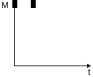
\includegraphics[width=0.4\textwidth]{\figpath/Model1_axes}}
		}
			\centerline{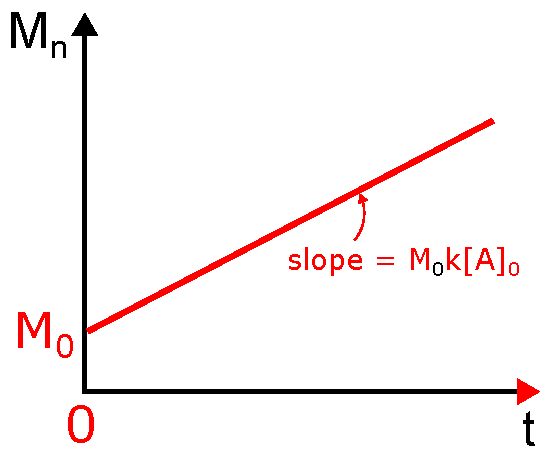
\includegraphics[width=0.3\textwidth]{\figpath/Model1_axes_catsoln}}
			
			(note the extra factor of $M_0$ in the slope, since the question asks for molecular weight rather than $N_n$!)
		
		\end{solution}		

\end{ctqs}
	

\begin{model}[Kinetics of Esterification Reactions]
\label{\labelbase:mdl:esterification}

	Esterification reactions used in polymer synthesis often proceed by the following mechanism (a Fischer esterification):
	
	\centerline{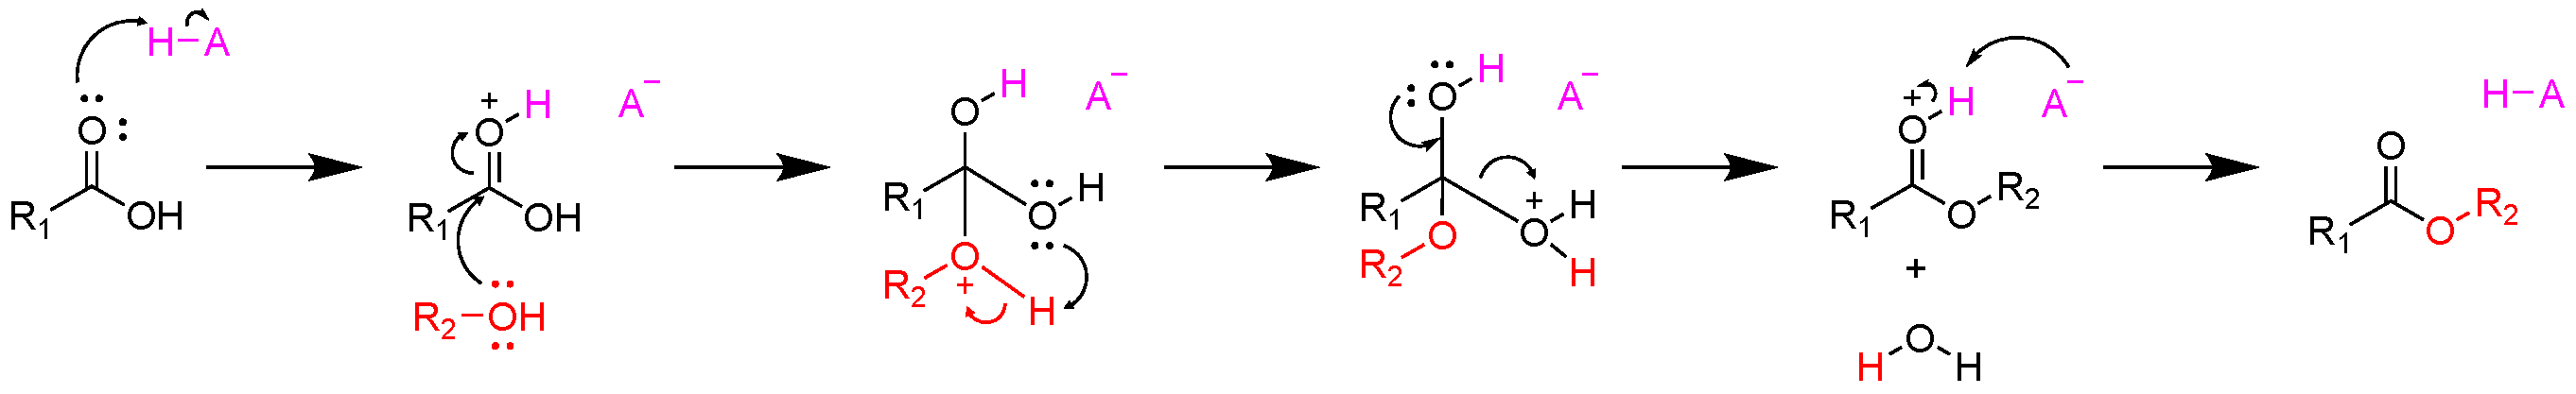
\includegraphics[width=\textwidth]{\figpath/Model2_mechanism}}

\end{model}

\begin{ctqs}

		\question In Activity 3.\ref{stepgrowth-chem}, you learned that esterification reactions typically require a carboxylic acid (R-COOH) and an alcohol (R-OH).  What \emph{additional} chemical species is required for the mechanism shown in Model \ref{\labelbase:mdl:esterification}?
		
			\begin{solution}[0.5in]{}
				An acid, H-A
			\end{solution}
		
		\question What happens to this additional reagent over the course of the reaction shown in Model \ref{\labelbase:mdl:esterification}?
		
			\begin{solution}[1.25in]{}
				It protonates the carboxylic acid, but is regenerated at the end of the mechanism (it is not used up or permanently bonded to the products).
			\end{solution}
		
		\question Based on your answer to the previous two questions, explain, in 1-2 complete sentences, why this reaction is referred to as an \emph{acid-catalyzed} esterification.
		
			\begin{solution}[1.75in]{}
				The acid catalyzes the reaction (it is required to make the reaction go but is not used up in the reaction since it is regenerated at the end).  Hence, it is an acid-catalyzed reaction.
			\end{solution}
			
		\question How many different molecules must come together for this reaction to proceed?
		
			\begin{solution}[0.5in]{}
				3 (carboxylic acid, alcohol, AND the acid HA)
			\end{solution}
		
		\question Explain, in 1-2 complete sentences, why the kinetics of this reaction should obey
		
			\begin{equation*}
				\frac{d[\text{COOH}]}{dt} = - k \text{[COOH][OH][HA]}
			\end{equation*}
			
			where [COOH], [OH], and [HA] are the concentrations of the carboxylic acid, alcohol, and acid catalyst, respectively.\label{\labelbase:ctq:fisherratelaw}
			
				\begin{solution}[1.25in]{}
					This is essentially a termolecular (or trimolecular) reaction that depends on three different reactants coming together.  If the concentration of any one of the reactants is decreased, it will be harder for these three reactants to find each other and the overall rate will slow down.  Thus, the rate law needs to contain the concentration of each of the species.
				\end{solution}
		
\end{ctqs}

\begin{infobox}
	In Fischer esterifications such as the reaction shown in Model \ref{\labelbase:mdl:esterification}, the acidic protons required to catalyze the reaction can be supplied either by an added acid, such as sulfuric acid, or by other carboxylic acids present in the reaction mixture.
\end{infobox}

\begin{ctqs}
	
	\question When the acidic proton is supplied by an added acid, we refer to the polymerization as a ``catalyzed'' step-growth polymerization.
	
		\begin{enumerate}
			\item Briefly explain why, if the acid is something like \ce{H2SO4}, it is reasonable to assume that [HA] is constant over the entire course of the reaction.
			
				\begin{solution}[0.75in]{}
					When the acid is NOT one of the reactants, it is not used up, so its concentration will not change.
				\end{solution}
			
			\item Critique or defend the following statement in 2-3 complete sentences:
			
				``The rate law for a catalyzed step-growth polymerization can effectively be simplified to $\frac{d[COOH]}{dt} = - k_c [COOH][OH]$, which means that the degree of polymerization will grows linearly with time.''
			
				\begin{solution}[1.75in]{}
				
				This statement is correct.  If [HA] is constant then we can just let $k_c = k[HA]$ and the expression from CTQ 10 reduces to the expression given in the statement.  This rate law then has exactly the same form as the rate law investigated in Model 1, so all of the same conclusions drawn in that analysis - including the linear growth of $N_n$ - hold.
				
				\end{solution}
				
		\end{enumerate}
		
	\question When the acidic proton is supplied by COOH groups from other monomers in the reaction mixture, we refer to the polymerization as an ``uncatalyzed'' step-growth polymerization.
	
		\begin{enumerate}
				
			\item  What rate law do you obtain if you replace [HA] in the expression given in CTQ \ref{\labelbase:ctq:fisherratelaw} with [COOH]?
			
				\begin{solution}[0.75in]	{}
					\begin{equation*}
						\frac{d[\text{COOH}]}{dt} = - k \text{[COOH]}^2\text{[OH]}
					\end{equation*}
				\end{solution}
		
			\item What happens to the concentration of COOH groups as the reaction progresses?
			
				\begin{solution}[0.75in]	{}
					[COOH] decreases as COOH groups are used up to form ester bonds.
				\end{solution}
			
			\item Based on your answers to the previous two questions, what do you expect to happen to the reaction rate as the reaction progresses?
			
				\begin{solution}[0.75in]	{}
					Because the rate depends on the square of the COOH concentration, the reaction rate will slow down substantially as the concentration of COOH groups decreases.
				\end{solution}
			
		\end{enumerate}
	
\end{ctqs}

\begin{infobox}\label{\labelbase:info:uncatintrate}
	The integrated rate law for uncatalyzed step-growth polymerizations is
	\begin{equation*}
		\frac{1}{[A]^2} = 2k_u t + \frac{1}{[A]_0^2}
	\end{equation*}
	which can be rewritten in terms of the extent of reaction as
	\begin{equation*}
		\frac{1}{(1-p)^2} = 1 + 2k_u [A]_0^2 t
	\end{equation*}
\end{infobox}

\begin{ctqs}

	\question Using this information, derive an expression for how the number average degree of polymerization, $N_n$, changes with time in an uncatalyzed step-growth polymerization.
	
		\begin{solution}[1.25in]{}
			\begin{equation*}
				N_n = \frac{1}{1-p} = \sqrt{1 + 2k_u [A]_0^2 t}
			\end{equation*}
		\end{solution}
		
	\question Based on the equation you derived in the previous question, sketch a plot of how the molecular weight of the polymers formed in an uncatalyzed step-growth polymerization should depend on the reaction time:
	
		\begin{solution}[2in]{		
			\centerline{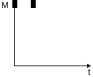
\includegraphics[width=0.4\textwidth]{\figpath/Model1_axes}}
		}
			\centerline{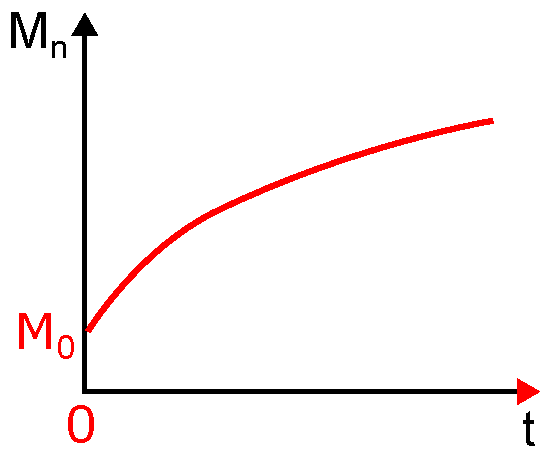
\includegraphics[width=0.4\textwidth]{\figpath/Model1_axes_uncatsoln}}
		
		\end{solution}		
		
	\question Which type of polymerization (catalyzed or uncatalyzed) do you expect to produce higher molecular weight polymers in a given amount of time?  Explain your group's reasoning in 2-3 complete sentences.
	
		\begin{solution}[2in]{}
		
			Generally, catalyzed reactions go more quickly than un-catalyzed reactions, so the catalyzed polymerization should produce higher molecular weight polymers in a given amount of time.  This is reflected in the expressions for $N_n$ derived above - for the catalyzed reaction, the degree of polymerization (and thus molecular weight) increase linearly with time, while for the uncatalyzed reaction, the square root dependence means that the increase in molecular weight slows down with time as more and more of the COOH is used up.
		\end{solution}

\end{ctqs}
	

\begin{exercises}

		\exercise In Model \ref{\labelbase:mdl:simple}, the ``A'' and ``B'' reactive groups were shown without depicting which species they were attached to.  However, these species could be on the ends of monomers, oligomers, or long polymer chains. %add graphic?
		What assumption has to be made about the reactivities of the functional groups on these different species for the rate law you proposed in CTQ \ref{\labelbase:ctq:proposeratelaw} (and the expression you derived for $N_n$ in CTQ \ref{\labelbase:ctq:catNn}) to correctly describe the kinetics of the entire reaction?  Explain your reasoning in 2-3 complete sentences.
		
			\begin{solution}{}
				For the rate law in CTQ \ref{\labelbase:ctq:proposeratelaw} to hold, we had to assume that all ``A'' and ``B'' reactive groups are equally likely to react, regardless of what species they are attached to (that is, an ``A'' group on a monomer has exactly the same probability of reacting as an ``A'' group on a polymer chain, etc.).  This is the \emph{principle of equal reactivity}, which is assumed in many analyses of polymerization kinetics.
			\end{solution}
			
		\exercise Derive the integrated rate law for stoichiometrically-balanced, catalyzed step-growth polymerizations (shown on page \pageref{\labelbase:infobox:catintegrated}) by doing the following: \label{\labelbase:exc:catinteratelaw}
		
			\begin{enumerate}
				\item Explain why, if the reaction is stoichiometrically balanced, it must be true that $[A]=[B]$ throughout the \emph{entire} course of the reaction.  Then, use this information to rewrite your expression from CTQ \ref{\labelbase:ctq:proposeratelaw} in terms of the concentration of A groups only.
				
					\begin{solution}{}
						Every reaction uses up one ``A'' and one ``B''.  If the numbers of A's and B's are equal to start, and they change in exactly the same way throughout the reaction, then their concentrations will be equal throughout the entire course of the reaction.
						
						Following this reasoning, we can assume $[A]=[B]$ and substitute $[B]$ with $[A]$ in the expression proposed in CTQ \ref{\labelbase:ctq:proposeratelaw}.  Doing so, we obtain
						\begin{equation*}
							\frac{d[A]}{dt} = -k[A]^2
						\end{equation*}
					\end{solution}
				
				\item Rearrange your equation into the form $f([A])\,d[A] = g(t)\,dt$ and then integrate both sides.
				
					\begin{solution}{}
						Rearranging the equation from the previous part, we obtain
						\begin{align*}
							\frac{1}{[A]^2}d[A] = -k dt
						\end{align*}
						Integrating both sides, we obtain
						\begin{align*}
							\int \frac{1}{[A]^2}d[A] &= \int -k dt \\
							\frac{-1}{[A]} &= -kt + C\\
							\frac{1}{[A]} &= kt + C
						\end{align*}
						where we have combined the integration constants from both sides into a single constant on the right-hand-side of the equation.
						
						(Note: students can also do this as a definite integral; in this case, the integration limits on the left side should be from $[A]_0$ to $[A](t)$ and on the right side should be from $0$ to $t$, and students will not need to do the step of applying the initial condition in the next question.)
					\end{solution}
				
				\item Finally, apply the initial condition that $[A]=[A]_0$ at $t=0$ and show that your answer rearranges to the form shown in the Information box on page \pageref{\labelbase:infobox:catintegrated}.
			\end{enumerate}
				
					\begin{solution}{}
						If $[A]=[A]_0$ at $t=0$, then we must have
						\begin{align*}
							\frac{1}{[A]_0} &= k\cdot 0 + C \\
							C &= \frac{1}{[A]_0}
						\end{align*}
						Putting this value of $C$ back into our equation, we have
						\begin{align*}
							\frac{1}{[A]} &= kt + \frac{1}{[A]_0} \\
							[A] &= \frac{1}{kt + \frac{1}{[A]_0}} \\
								&= \frac{[A]_0}{kt[A]_0 + 1}
						\end{align*}
						which is equivalent to the expression given on page \pageref{\labelbase:infobox:catintegrated}, as desired. 
						
					\end{solution}
			
		\exercise Extend the process from the above question to derive the integrated rate law for stoichiometrically-balanced, un-catalyzed step-growth polymerizations (shown on page \pageref{\labelbase:info:uncatintrate}).
				
					\begin{solution}{}
						For the un-catalyzed polymerization, 
						\begin{equation*}
							\frac{d[\text{COOH}]}{dt} = - k \text{[COOH]}^2\text{[OH]}
						\end{equation*}
						Letting $[COOH]\equiv [A]$ and $[OH]\equiv[B]$, and setting $[A]=[B]$ following the same reasoning as in the previous question, we obtain
						\begin{equation*}
							\frac{d[A]}{dt} = - k [A]^2[B] = -k[A]^3
						\end{equation*}
						Rearranging and integrating, we obtain
						\begin{align*}
							\frac{1}{[A]^3} d[A] &= -k dt \\
							\int \frac{1}{[A]^3} d[A] &= \int -k dt \\
							\frac{-1}{2[A]^2} &= -kt + C\\
							\frac{1}{2[A]^2} &= kt + C
						\end{align*}
					\end{solution}
					\begin{solution}{}
						Applying the initial condition $[A]_0=0$ at $t=0$, we obtain
						\begin{align*}
							\frac{1}{2[A]_0^2} &= C 
						\end{align*}
						so
						\begin{align*}
							\frac{1}{2[A]^2} &= kt + \frac{1}{2[A]_0^2} \\
							\frac{1}{[A]^2} &= 2kt + \frac{1}{[A]_0^2}
						\end{align*}
						as desired.
						
						Note: the question did not specifically ask for the expression in terms of $p$, but again, $p=1-\frac{[A]}{[A]_0}$ so
						\begin{align*}
							p &= 1-\frac{[A]}{[A]_0} \\
							1-p &= \frac{[A]}{[A]_0} \\
							\frac{1}{1-p} &= \frac{[A]_0}{[A]}\\
							\frac{1}{(1-p)^2} &= \left(\frac{[A]_0}{[A]}\right)^2\\
							 &= [A]_0^2\left(2k_u t + \frac{1}{[A]_0^2}\right)\\
								&= 1+ 2k_u[A]_0^2 t
						\end{align*}
						as desired.
					\end{solution}
				
				% could also the rate law for a stoichiometrically-\emph{unbalanced} catalyzed step-growth polymerization that starts with A and B reactive group concentrations of $[A]_0$ and $[B]_0$, respectively....
			
		%\exercise The kinetic scheme shown in Model \ref{\labelbase:mdl:simple} is somewhat over-simplified.  In practice, most step-growth reactions can be thought of as proceeding through formation of a ``caged'' intermediate, where the A and B reactive groups ...
		
		%\exercise add a question about the relative kinetics of ring formation, and why step-growth polyms are usually performed in bulk (e.g. to promote bimolecular rxn over unimolecular rxn)?
		
\end{exercises}
	
\end{activity}